\documentclass[solutions]{esg8012pset} 
  \usepackage{amsmath}
  \usepackage{amssymb}
  \usepackage{enumerate}
  \usepackage{graphicx}
  \providecommand{\uvec}[1]{{\hat{\bf{#1}}}}
\classname{Physics 8.012} 
\semester{Fall 2010} 
\problemsetnumber{1} 
\date{September 8} 
\duedate{Friday, September 17} 
\readingassignment{Chapter One: Kleppner and Kolenkow, \emph {An Introduction to Mechanics}} 
\begin{document}
\section*{Problem 1: Fermi Problem (This problem is hard and should be a challenge.)}
\subsection*{Problem}
  One of the moons of Jupiter, Europa, is reported to have its surface covered by an ocean of water
  which is 100 km deep.  The outermost 8 km are frozen as ice. The radius of Europa is
  approximately 1/4 the radius of the earth. Estimate the pressure at the bottom of Europa's ocean.
  (Note: there is some speculation that the combination of internal heat and water makes the ocean
  of Europa the best candidate in the solar system outside the earth for organized life to evolve.)
\subsection*{Solution}
  Pressure at bottom of ocean?  Force / Area.  $(7.5\cdot 10^{21}\text{ N}) / (2.7 \cdot 10^{13}\text{ m}^2) \approx 3 \cdot 10^8$ N / m$^2$
  \begin{itemize}
    \item Force: Mass $\cdot$ Acceleration (due to gravity). $(3 \cdot 10^{21}\text{ kg}) \cdot (2.5\text{m / s}^2) \approx 7.5\cdot 10^{21}$ N
      \begin{itemize}
        \item Mass: density $\cdot$ volume.  $(10^{12}\text{ kg / km}^3) \cdot (3 \cdot 10^9\text{ km}^3) \approx 3 \cdot 10^{21}$ kg
          \begin{itemize}
            \item Density: the density of ice is about the same as that of water, 1 g / cm$^3$, or $10^{12}$ kg / km$^3$
            \item Volume: The volume is the difference of the volumes of the spheres, or $\frac{4}{3}\pi (R^3 - r^3)$, or (approximating $\pi$ as 3), $4((1600\text{ km})^3 - (1600\text{ km})^3) \approx 3 \cdot 10^9$ km$^3$
          \end{itemize}
        \item Acceleration due to gravity: Since mass is linear in volume, and volume is cubic in radius, Europa has about $\frac{1}{4^3}$ the mass of earth, and since the force of gravity is linear in mass / the square of the radius, the force of gravity on Europa is about $\frac{4^2}{4^3} = \frac{1}{4}$ that on earth, so it's about 2.5 m/s$^2$  Alternatively, by dimensional analysis, the acceleration due to gravity is linear in m$^{-1}$, so the acceleration due to gravity on Europa is about $\frac{1}{4}$ that of earth.
      \end{itemize}
    \item Area: $4\pi r^2$.  Let $\pi \approx 3$, so area is about $2.7 \cdot 10^{13}$ m$^2$
      \begin{itemize}
        \item Radius: $\frac{1}{4}$ radius of earth, less 100 km, so about 1500 km (since, according to google, the radius of earth is 6378.1 km)
      \end{itemize}
  \end{itemize}
  \vspace{2em}
  \noindent Alternatively: \par
  Pressure $ = \frac{F}{A} = \frac{mg}{A} = \frac{\rho Vg}{A} = \frac{\rho h A g}{A} = \rho h g = (10^{12}\text{ kg / km}^3)(100\text{ km})(2.5\text{ m / s}^2) \approx 3\cdot 10^8$ N / m$^2$
  \begin{itemize}
    \item Density: the density of ice is about the same as that of water, 1 g / cm$^3$, or $10^{12}$ kg / km$^3$
    \item Height: the height is about 100 km
    \item Acceleration due to gravity: Since mass is linear in volume, and volume is cubic in radius, Europa has about $\frac{1}{4^3}$ the mass of earth, and since the force of gravity is linear in mass / the square of the radius, the force of gravity on Europa is about $\frac{4^2}{4^3} = \frac{1}{4}$ that on earth, so it's about 2.5 m/s$^2$  Alternatively, by dimensional analysis, the acceleration due to gravity is linear in m$^{-1}$, so the acceleration due to gravity on Europa is about $\frac{1}{4}$ that of earth.
  \end{itemize}
\section*{Problem 2: Kinematics-One Dimension}
\subsection*{Problem}
  A bus leaves a stop at MIT and accelerates at a constant rate for 5 seconds. During this time the
  bus traveled 25 meters. Then the bus traveled at a constant speed for 15 seconds. Then the driver
  noticed a red light 18 meters ahead and slams on the brakes. Assume the bus decelerates at a
  constant rate and comes to a stop some time later just at the light.
  \begin{enumerate}[a)]
    \item What was the initial acceleration of the bus?
    \item What was the velocity at the bus after 5 seconds?
    \item What was the braking acceleration of the bus? Is it positive or negative?
    \item How long did the bus brake?
    \item What was the distance from the bus stop to the light?
    \item Make a graph of the position vs. time for the entire trip.
    \item Make a graph of the velocity vs. time for the entire trip.
    \item Make a graph of the acceleration vs. time for the entire trip.
  \end{enumerate}
\subsection*{Solution}
  \begin{enumerate}[a)]
    \item Since $\displaystyle \int_{0}^{5}\int_{0}^{t} a \,d{t'}\,d{t} = 25\ \text{m}$, $\frac{1}{2}a \cdot 5^2 = 25$, so $2$ m / s$^2$.
    \item 10 m / s
    \item $\frac{1}{2}at^2 = 18$ m, and $at = 10$ m / s, so $t = 3.6$ s, and $a = 2.\overline{7}$ m / s$^2$.  It is negative.
    \item 3.6 s
    \item $25 + 10 \cdot 15 + 18 = 193$ m
    \item 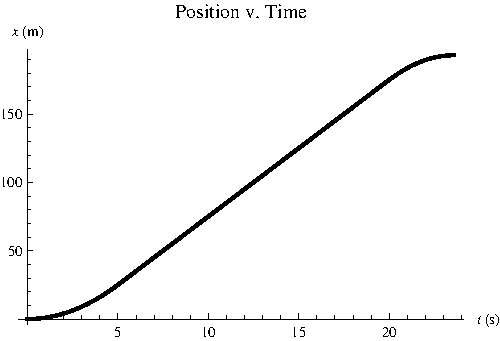
\includegraphics[width=0.85\textwidth]{ps01_Plot_1}
    \item 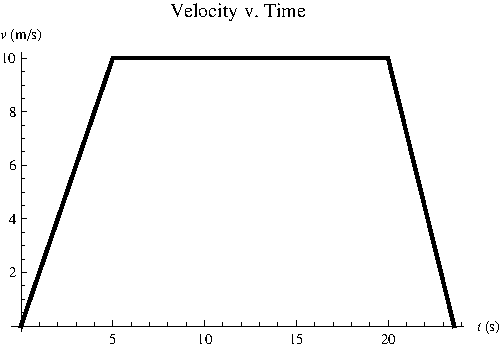
\includegraphics[width=0.85\textwidth]{ps01_Plot_2}
    \item 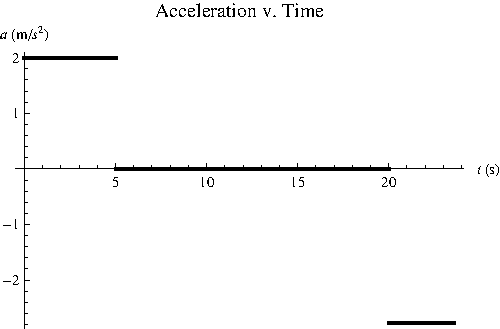
\includegraphics[width=0.85\textwidth]{ps01_Plot_3}
  \end{enumerate}
\section*{Problem 3: Kinematics-One Dimension}
\subsection*{Problem}
  You are a running as fast as you can at a constant velocity, $v_p$, trying to catch a bus that is at rest
  at a bus stop. When you are still a distance $b$ away from the bus stop, the bus starts to accelerate
  at a constant rate $a_\text{bus}$.
  \begin{enumerate}[a)]
    \item What is the minimum velocity that you need to run at in order to just catch the bus?
    \item Draw graphs showing the motion of the bus and yourself.
    \item How long did it take to catch the bus?
  \end{enumerate}
\subsection*{Solution}
  \begin{enumerate}[a)]
    \item If you just catch the bus after time $t$, then $v_p = a_{bus}t$.  If you catch the bus after time $t$, $v_p t = b + \frac{1}{2}a_{bus}t^2 = b + \frac{1}{2}v_p t$, so $t = \sqrt{2\frac{b}{a_{bus}}}$.  Then $v_p = \sqrt{2 b a_{bus}}$.
    \item 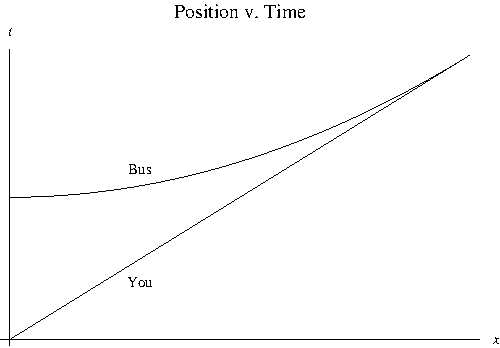
\includegraphics[width=0.85\textwidth]{ps01_Plot_4}
    \item $\sqrt{2\frac{b}{a_{bus}}}$
  \end{enumerate}
\section*{Problem 4: K\&K 1.7}
\subsection*{Problem}
  Let $\uvec a$ and $\uvec b$ be unit vectors in the $xy$ plane making angles $\theta$ and $\phi$ with the $x$ axis,
  respectively. Show that $\uvec a = \cos\theta\uvec i + \sin\theta\uvec j$, $\uvec b = \cos\phi\uvec i + \sin\phi\uvec j$, and using vector algebra prove
that $\cos(\theta -\phi ) = \cos\theta \cos\phi + \sin\theta \sin\phi$.
\subsection*{Solution}
  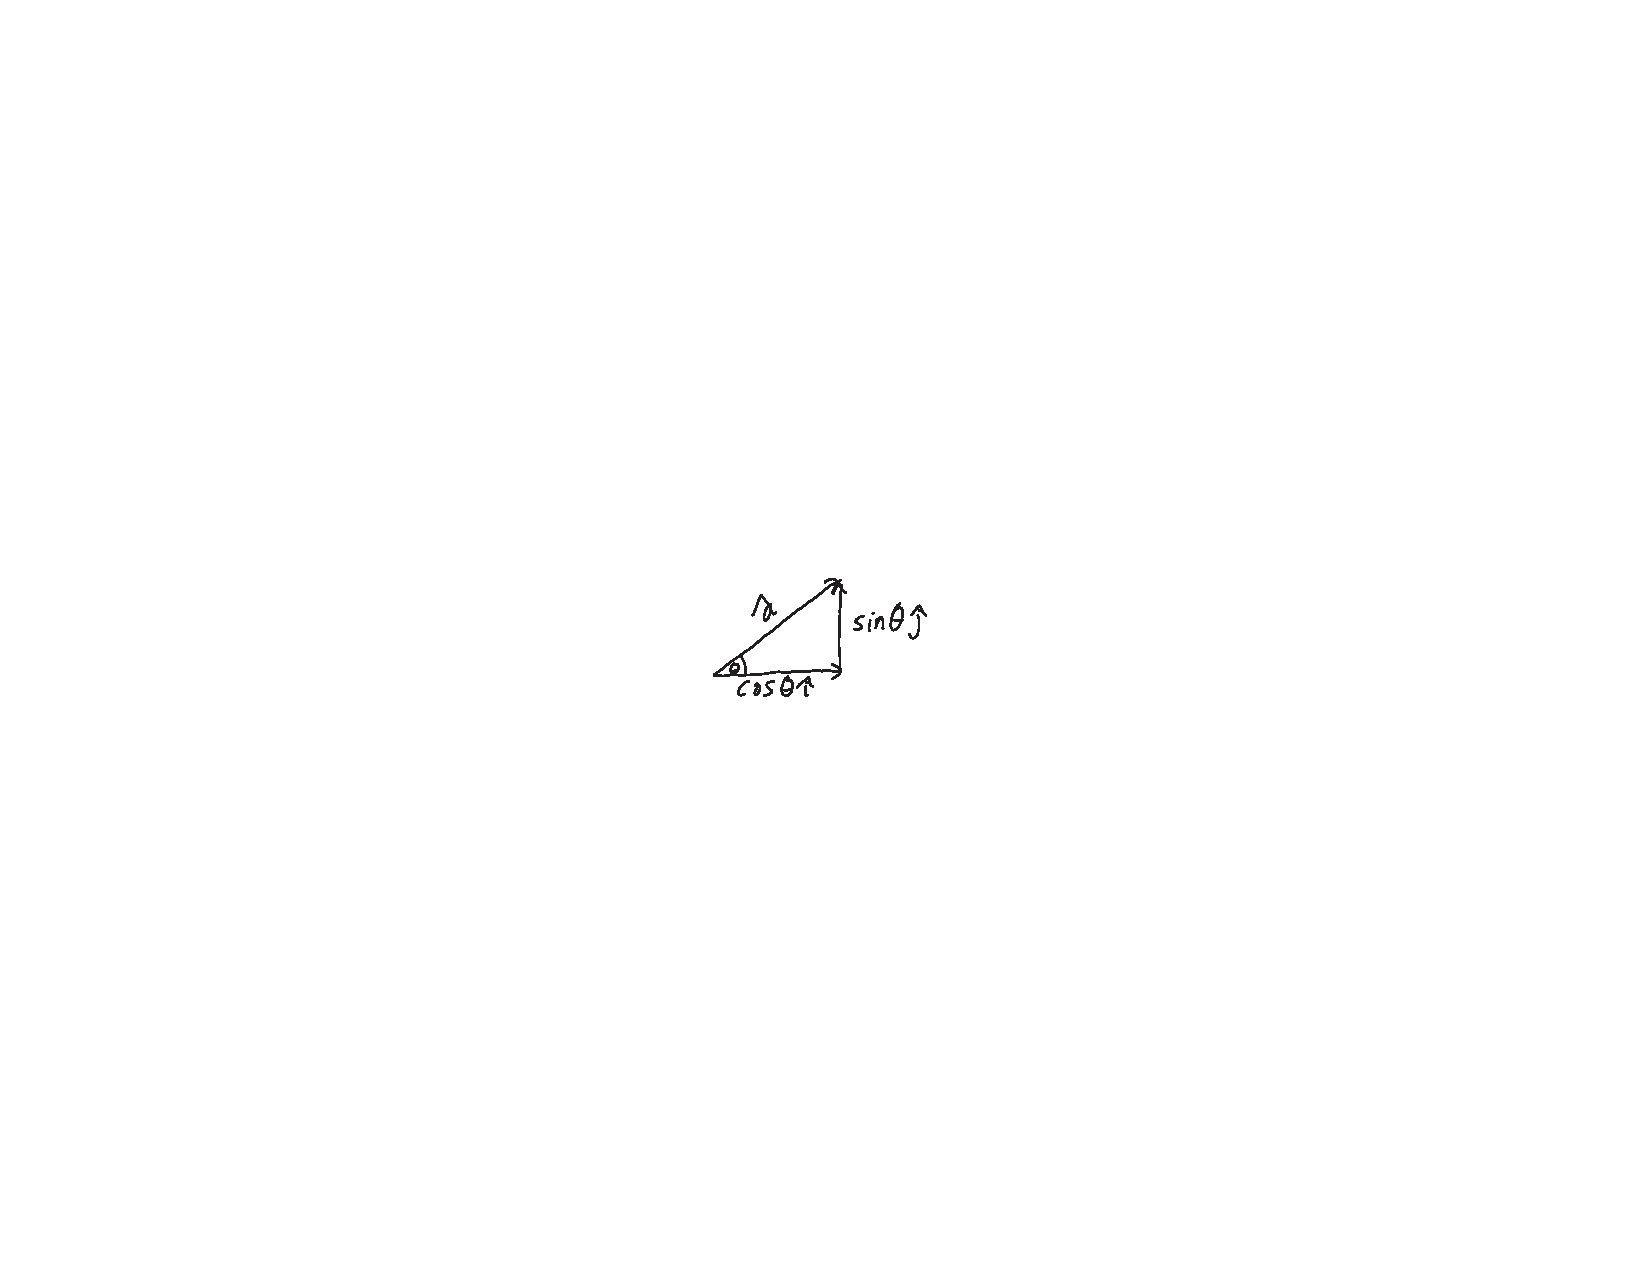
\includegraphics[width=0.85\textwidth]{ps01_Diagram_1}

  As seen in the diagram, by the definition of $\cos$ and $\sin$, $\uvec a = \cos\theta\uvec i + \sin\theta\uvec j$.  By relabeling, $\uvec b = \cos\phi\uvec i + \sin\phi\uvec j$.
  \begin{center}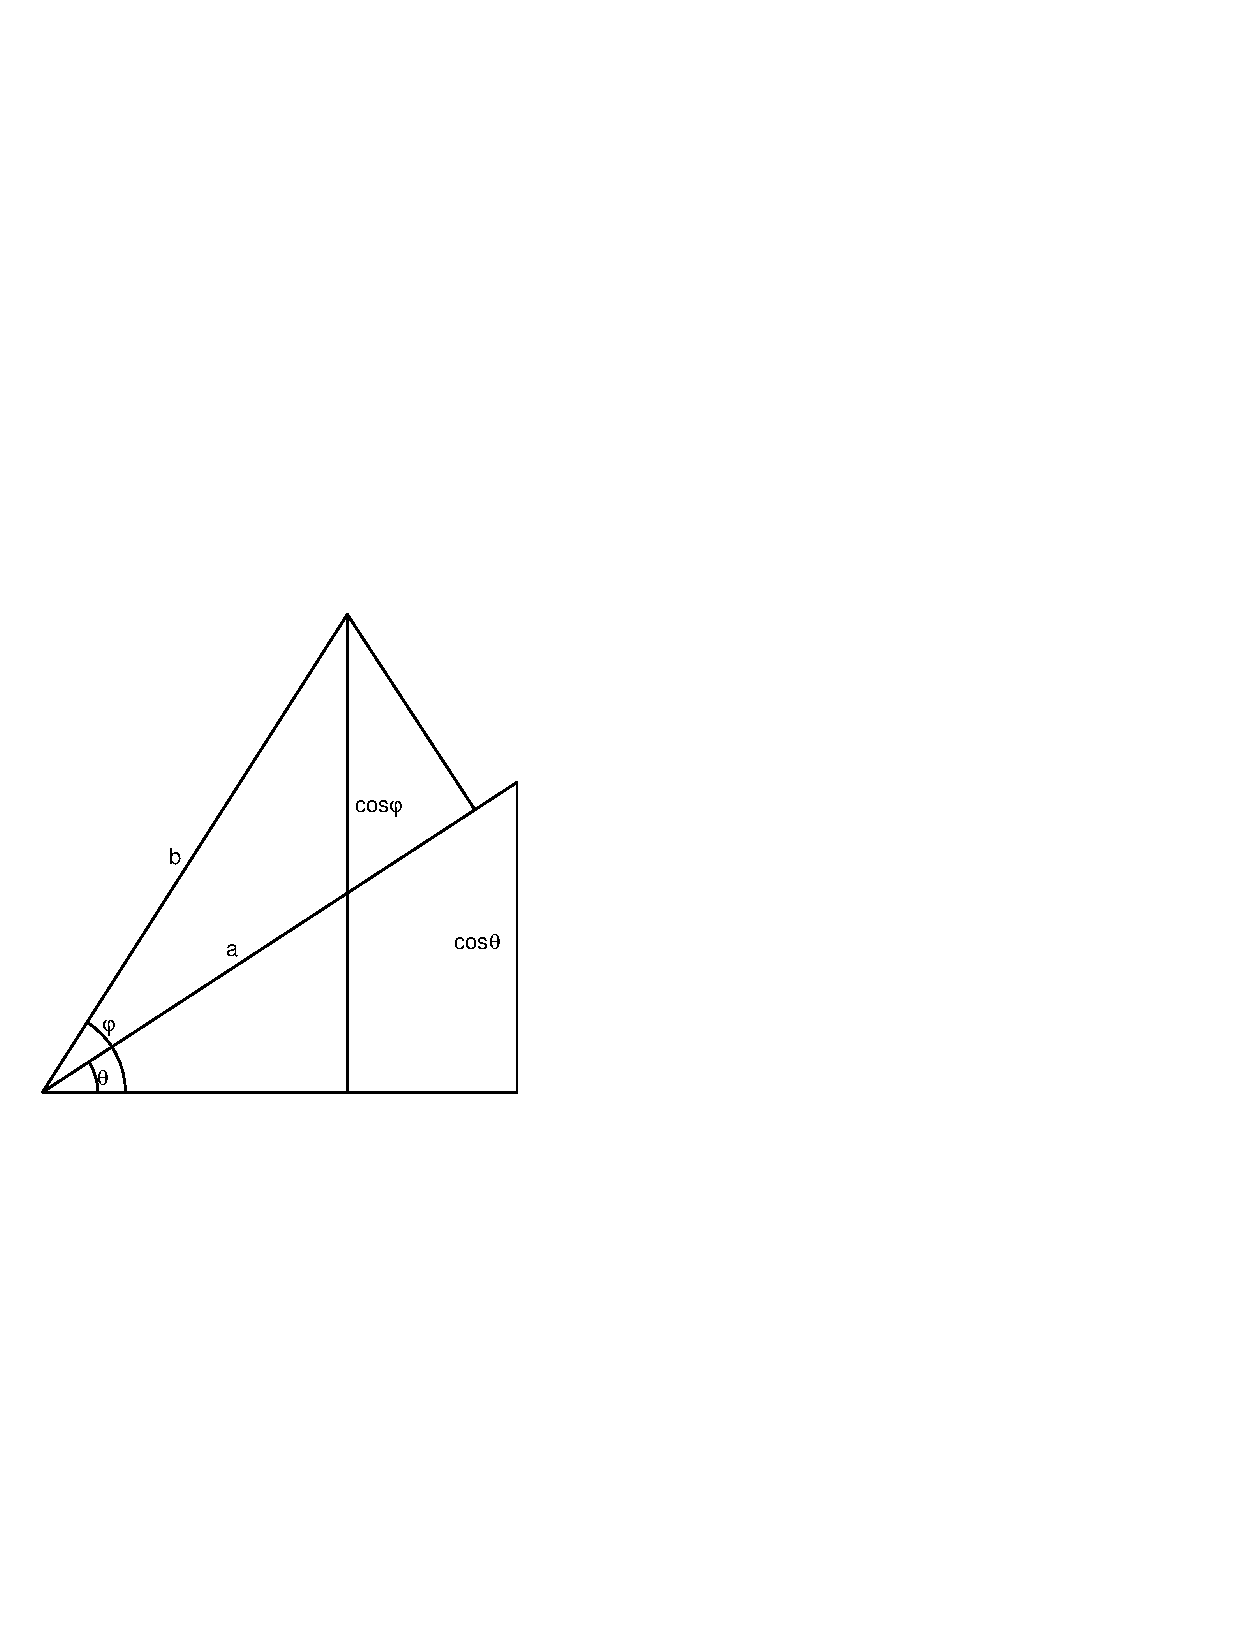
\includegraphics[width=.33\textwidth]{ps01_Diagram_2}\end{center}

  By the definition of $\cos$, $\cos(\phi - \theta) = \vec a \cdot \vec b$ (since $\vec a$ and $\vec b$ are unit vectors).  Then $\cos(\theta - \phi) = \cos(\phi - \theta) = \cos\theta\cos\phi + \sin\theta\sin\phi$.
\section*{Problem 5: K\&K 1.12}
\subsection*{Problem}
  The acceleration of gravity can be measured by projecting a body upward and measuring the
  time that it takes to pass two given points in both directions. Show that if the time the body takes
  to pass a horizontal line $A$ in both directions is $T_A$ , and the time to go by a second line $B$ is $T_B$,
  then, assuming that the acceleration is constant, its magnitude is
  $$g = \frac{8h}{T_A^2 - T_B^2}$$
  \begin{center}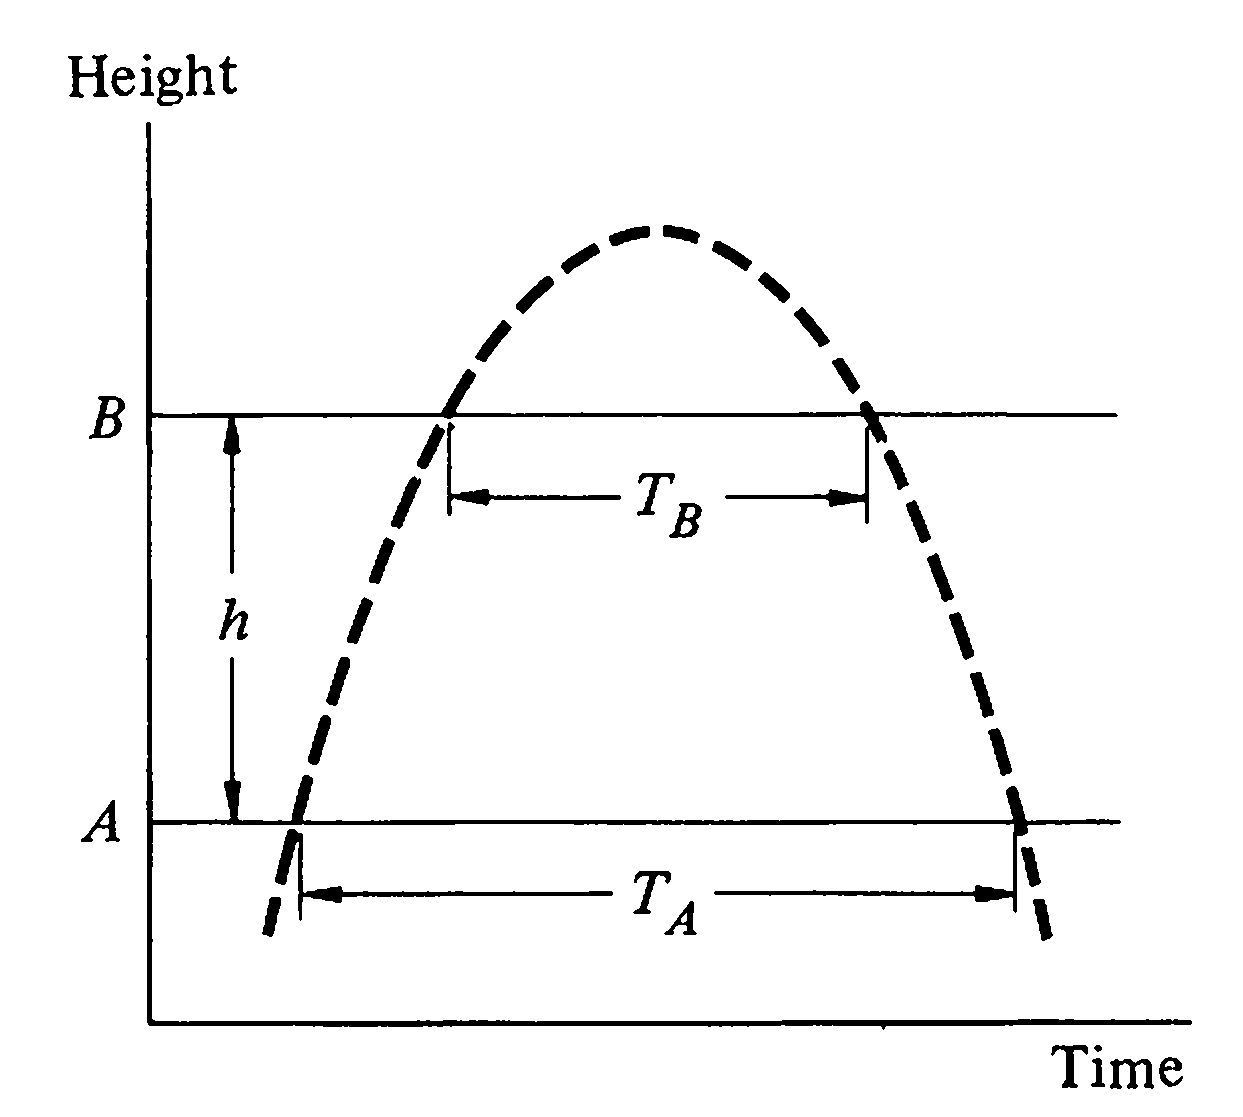
\includegraphics[width=0.35\textwidth]{ps01_1}\end{center}
\subsection*{Solution}
  Since acceleration is constant downwards, $\frac{\partial^2 y}{\partial t^2} = g$.  Then $y(t) = y_0 + v_0 t + \frac{1}{2} g t^2$.  It is given that for some $t$, $y\left(t + \frac{T_B}{2}\right) = y\left(t - \frac{T_B}{2}\right)$, and $y\left(t + \frac{T_A}{2}\right) - y\left(t + \frac{T_B}{2}\right) = h$.  Translate the function such that this $t = 0$.  Then $v_0 \frac{T_B}{2} + \frac{1}{2} g \left(\frac{T_B}{2}\right)^2 = -v_0 \frac{T_B}{2} + \frac{1}{2} g \left(\frac{T_B}{2}\right)^2$.  Equivalently, $v_0 = 0$.

  Then, the other conditions states that $\frac{1}{2} g\left(\left(\frac{T_A}{2}\right)^2 - \left(\frac{T_B}{2}\right)^2\right) = h$.  Solving for $g$, $g = \frac{8h}{T_A^2 - T_B^2}$.
\section*{Problem 6: K\&K 1.15}
\subsection*{Problem}
  By relative velocity we mean velocity with respect to a specified coordinate system. (The term
  velocity, alone, is understood to be relative to the observer's coordinate system.)
  \begin{center}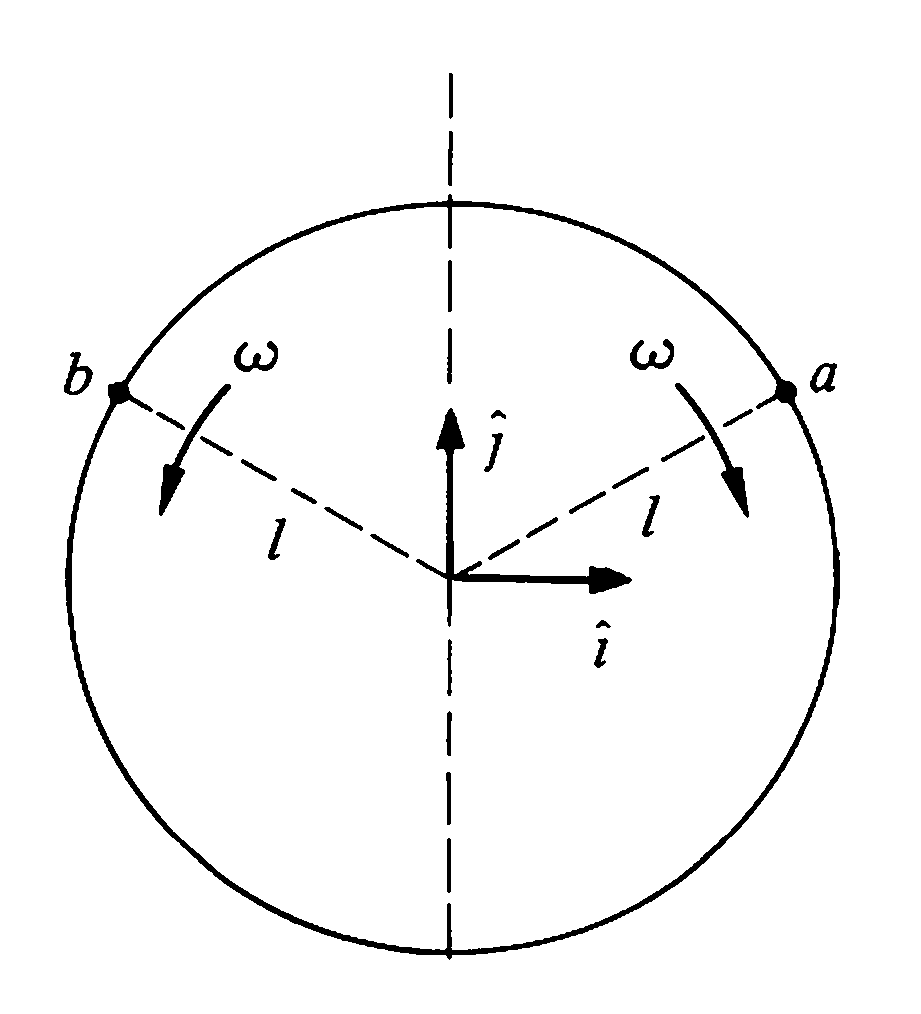
\includegraphics[width=0.35\textwidth]{ps01_2}\end{center}
  \begin{enumerate}[a.]
    \item A point is observed to have velocity $\vec v_A$ relative to coordinate system $A$. What is its
  velocity relative to coordinate system $B$, which is displaced from system $A$ by distance $\vec R$? ($\vec R$ can change in time.)
    \item Particles $a$ and $b$ move in opposite directions around a circle with angular velocity $\omega$,
  as shown. At $t = 0$ they are both at the point $\vec r = l\hat j$, where $l$ is the radius of the circle.
  Find the velocity of $a$ relative to $b$.
  \end{enumerate}
\subsection*{Solution}
  \begin{enumerate}[a.]
    \item The position vectors are related by
      \begin{equation} \vec r_B = \vec r_A - \vec R. \label{eq:1.15-rel_frame_vector}\end{equation}
      Then velocities are related by the taking derivatives, (law of addition of velocities)
      \begin{equation} \vec v_B = \vec v_A - \vec V. \label{eq:1.15-particle_A_vector}\end{equation} %Assuming $\left\| \vec v_A\right\|$ and $\left\| \frac{\partial \vec R}{\partial t} \right\|$   are negligible compared to $c$, the velocity relative to coordinate system $B$ is $\frac{\partial\vec v_A}{\partial t} - \frac{\partial \vec R}{\partial t}$.
    \item Let's choose two reference frames; frame B is centered at particle b, and frame A is centered at the center of the circle in the figure below.
      \begin{center}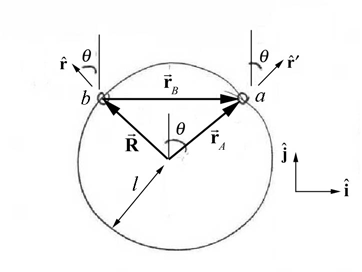
\includegraphics{ps01_Solution_06_01}\end{center}
      Then the relative position vector between the origins of the two frames is given by
      \begin{equation} \vec R = l\hat r. \label{eq:1.15-rel_origin_vector}\end{equation}
      The position vector of particle a relative to frame A is given by
      \begin{equation} \vec r_A = l\vec r'. \label{eq:1.15-particle_rel_A_vector}\end{equation}
      The position vector of particle b in frame B can be found by substituting Eqs. \ref{eq:1.15-particle_rel_A_vector} and \ref{q:1.15-rel_origin_vector} into Eq. \ref{eq:1.15-rel_frame_vector},
      \begin{equation} \vec r_B = \vec r_A - \vec R = l\hat r' - l\hat r. \label{eq:1.15-pos_b_in_B} \end{equation}
      We can decompose each of the unit vectors $\hat r$ and $\hat r'$ with respect to the Cartesian unit vectors $\hat i$ and $\hat j$ (see figure)
      \begin{align}
        \hat r & = -\sin\theta \hat i + \cos\theta \hat j \label{eq:1.15-cartesian_r_hat} \\
        \hat r' & = \sin\theta \hat i + \cos\theta \hat j \label{eq:1.15-cartesian_r_hat'}
      \end{align}
      Then Eq. \ref{eq:1.15-pos_b_in_B} giving the position vector of particle b in frame B becomes
      \begin{equation}
        \vec r_B = l\hat r' - l\hat r = l(\sin\theta \hat i + \cos\theta + \hat j) - l(-\sin\theta \hat i + \cos\theta \hat j) = 2l\sin\theta \hat i. \label{eq:1.15-pos_b_in_B_cartesian}
      \end{equation}
      In order to find the velocity vector of particle a in frame B (i.e., with respect to particle b), differentiate Eq. \ref{eq:1.15-pos_b_in_B_cartesian}
      \begin{equation}
        \vec v_B = \frac{d}{dt}(2l\sin\theta) \hat i = (2l\cos\theta)\frac{d\theta}{dt}\hat i = 2\omega l \cos\theta \hat i.
      \end{equation}
  \end{enumerate}
\section*{Problem 7: K\&K 1.19}
\subsection*{Problem}
  A bicycle wheel of radius $a$ is rolling in a straight line without slipping at a constant horizontal
  velocity $V$. A bead is fixed to a spoke a distance $b$ from the center of the wheel.
  \begin{center}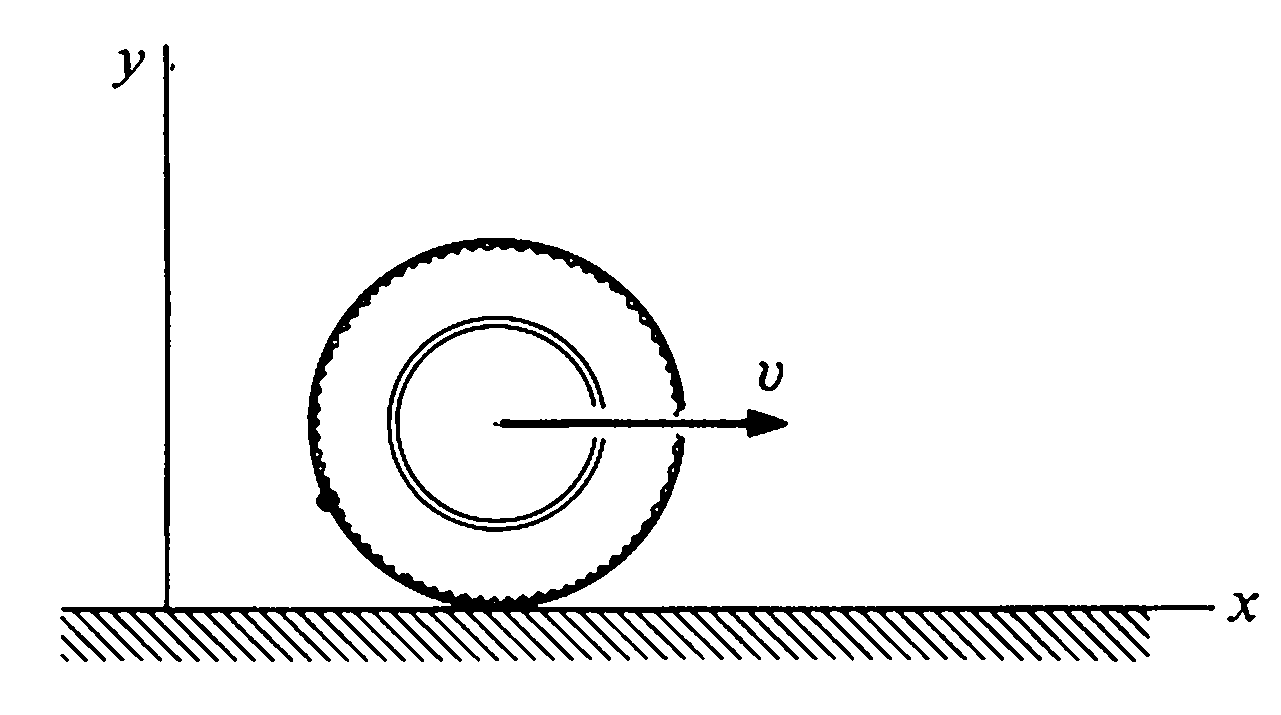
\includegraphics[width=0.5\textwidth]{ps01_3}\end{center}
  \begin{enumerate}[a)]
    \item Find the position and velocity of the bead as a function of time as seen by an observer located
  at the center of the wheel and moving with the wheel. Make sure you use appropriate unit
  vectors in your answer.
    \item What is the position and velocity of the observer at the center of the wheel as seen by an
  observer fixed to the ground. Assume at $t = 0$ that the center of the wheel is directly over the
  observer fixed to the ground. Make sure you use appropriate unit vectors in your answer.
    \item What is the relation between the angular velocity of the wheel, $\omega$, and the horizontal velocity, $V$, of the wheel?
    \item Find the position and velocity of the bead as a function of time as seen by the observer fixed
  to the ground. Make sure you use appropriate unit vectors in your answer.
  \end{enumerate}
\subsection*{Solution}
  \begin{enumerate}[a)]
    \item The angular velocity of the wheel, $\omega = 2\pi \frac{V}{2\pi a} = \frac{V}{a}$.  Then the position of the bead is given by $\vec r = b\cos\left(\frac{V}{a}t\right)\hat i + b\sin\left(\frac{V}{a}t\right)\hat j$.  $\frac{\partial \vec r}{\partial t} = -b\frac{V}{a}\sin\left(\frac{V}{a}t\right)\hat i + b\frac{V}{a}\cos\left(\frac{V}{a}t\right)\hat j$
    \item $\frac{\partial \vec x}{\partial t} = V\hat i$ and $\vec x = V t\hat i$
    \item $\omega = 2\pi \frac{V}{2\pi a} = \frac{V}{a}$
    \item $\vec r_G = \left(b\cos\left(\frac{V}{a}t\right) + Vt\right)\hat i + b\sin\left(\frac{V}{a}t\right)\hat j$ and $\frac{\partial \vec r_G}{\partial t} = \left(-b\frac{V}{a}\sin\left(\frac{V}{a}t\right) + V\right)\hat i + b\frac{V}{a}\cos\left(\frac{V}{a}t\right)\hat j$
  \end{enumerate}
\section*{Problem 8: K\&K 1.20}
\subsection*{Problem}
  A particle moves outward along a spiral. Its trajectory is given by
  $r = A\theta$, where $A$ is a constant, $A = (1/\pi )$ m $\cdot$ rad$^{-1}$.  $\theta$ increases in time according to $\theta =\alpha t^2 / 2$, where $\alpha$ is a constant.
  \begin{enumerate}[a.]
    \item Sketch the motion, and indicate the approximate velocity and acceleration at a few
  points.
    \item Show that the radial acceleration is zero when $\theta =1/\sqrt{2}$ rad.
    \item At what angles do the radial and tangential accelerations have equal magnitude?
  \end{enumerate}
\subsection*{Solution}
  \begin{enumerate}[a.]
    \item 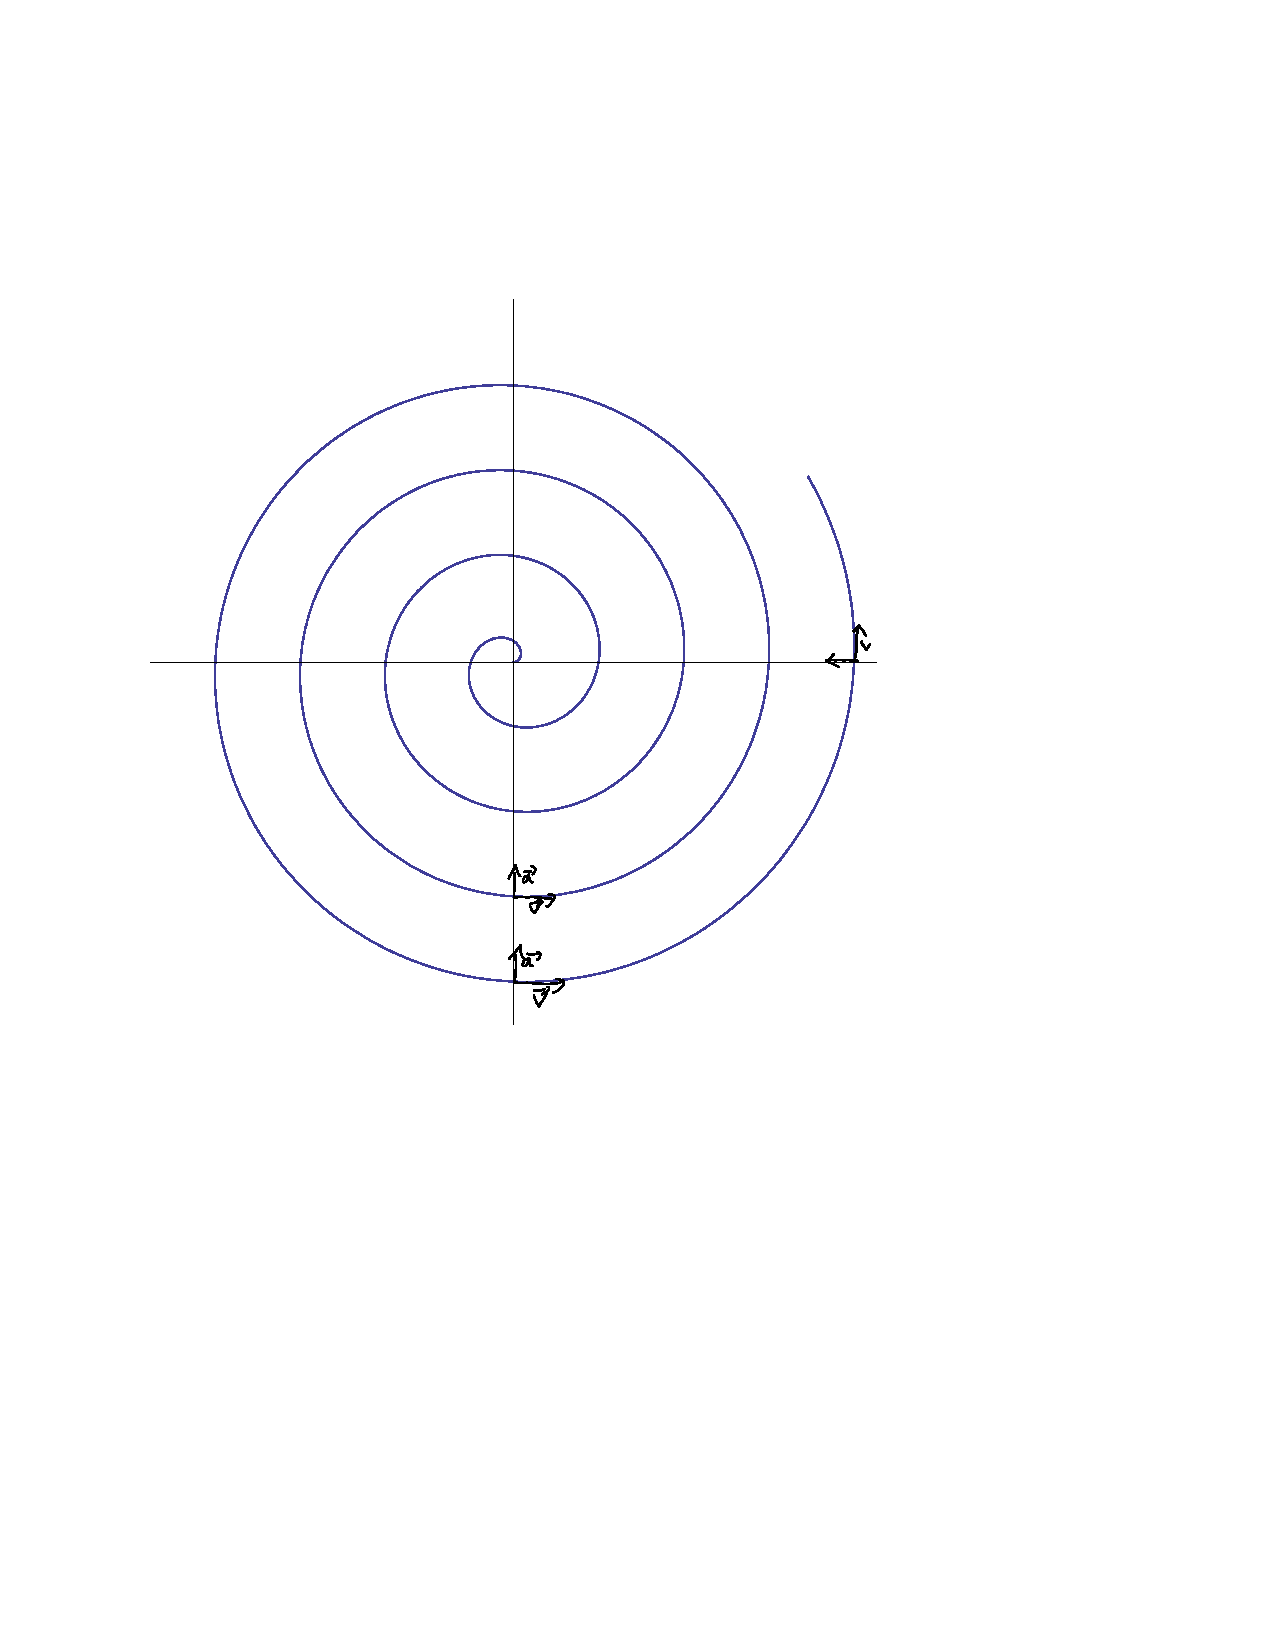
\includegraphics[width=0.85\textwidth]{ps01_Diagram_3}
    \item \begin{align*}
            \vec r(t) & = A\frac{\alpha t^2}{2} \hat r \\
            \vec \theta(t) & = \frac{\alpha t^2}{2} \hat\theta \\
            \\
            \frac{\partial \hat r}{\partial t} & = \alpha t \hat \theta \\
            \frac{\partial \hat \theta}{\partial t} & = -\alpha t \hat r \\
            \\
            \frac{\partial \vec r}{\partial t} & = \frac{A\alpha}{2}\left( 2t\hat r + t^2\frac{\partial \hat r}{\partial t}\right) \\
            & = \frac{A\alpha}{2}\left( 2t\hat r + \alpha t^3 \hat \theta\right) \\
            \\
            \frac{\partial^2 \vec r}{\partial t^2} & = \frac{A\alpha}{2}\frac{\partial}{\partial t}\left( 2t\hat r + \alpha t^3 \hat \theta\right) \\
            & = \frac{A\alpha}{2}\left( 2\hat r + 2t\frac{\partial \hat r}{\partial t} + 3\alpha t^2 \hat \theta + \alpha t^3\frac{\partial \hat \theta}{\partial t}\right) \\
            & = \frac{A\alpha}{2}\left( 2\hat r + 2t\alpha t \hat \theta + 3\alpha t^2 \hat \theta + \alpha t^3(-\alpha t \hat r)\right) \\
            & = \frac{A\alpha}{2}\left( 2\hat r + 2\alpha t^2 \hat \theta + 3\alpha t^2 \hat \theta - \alpha^2 t^4\hat r\right) \\
            & = \frac{A\alpha}{2}\left( \left(2- 4\left(\frac{\alpha t^2}{2}\right)^2\right)\hat r + 5\alpha t^2\hat \theta \right) \\
            & = A\alpha\left( \left(1- 2\theta^2\right)\hat r + 5\theta\hat \theta \right) \\
            & = A\alpha\left( \left(1- 2\cdot\frac{1}{2}\right)\hat r + \frac{5}{\sqrt{2}}\hat \theta \right) \\
            & = \frac{5A\alpha}{\sqrt{2}}\hat \theta
          \end{align*} \par
          Since all of the coefficient of $\hat r$ is 0, the radial acceleration is 0.
    \item  The radial and tangential accelerations have equal magnitudes if $1- 2\theta^2 = 5\theta$.  That is, $\theta \equiv \frac{-5\pm\sqrt{33}}{4}\pmod{2\pi}$.
  \end{enumerate}
\section*{Problem 9: K\&K 1.21}
\subsection*{Problem}
  A person throws a rock from the top of a hill. The hill slopes downward uniformly at angle $\phi$. At
  what angle $\theta$ from the horizontal should the person throw the rock so that it has the greatest
  range?
  \begin{center}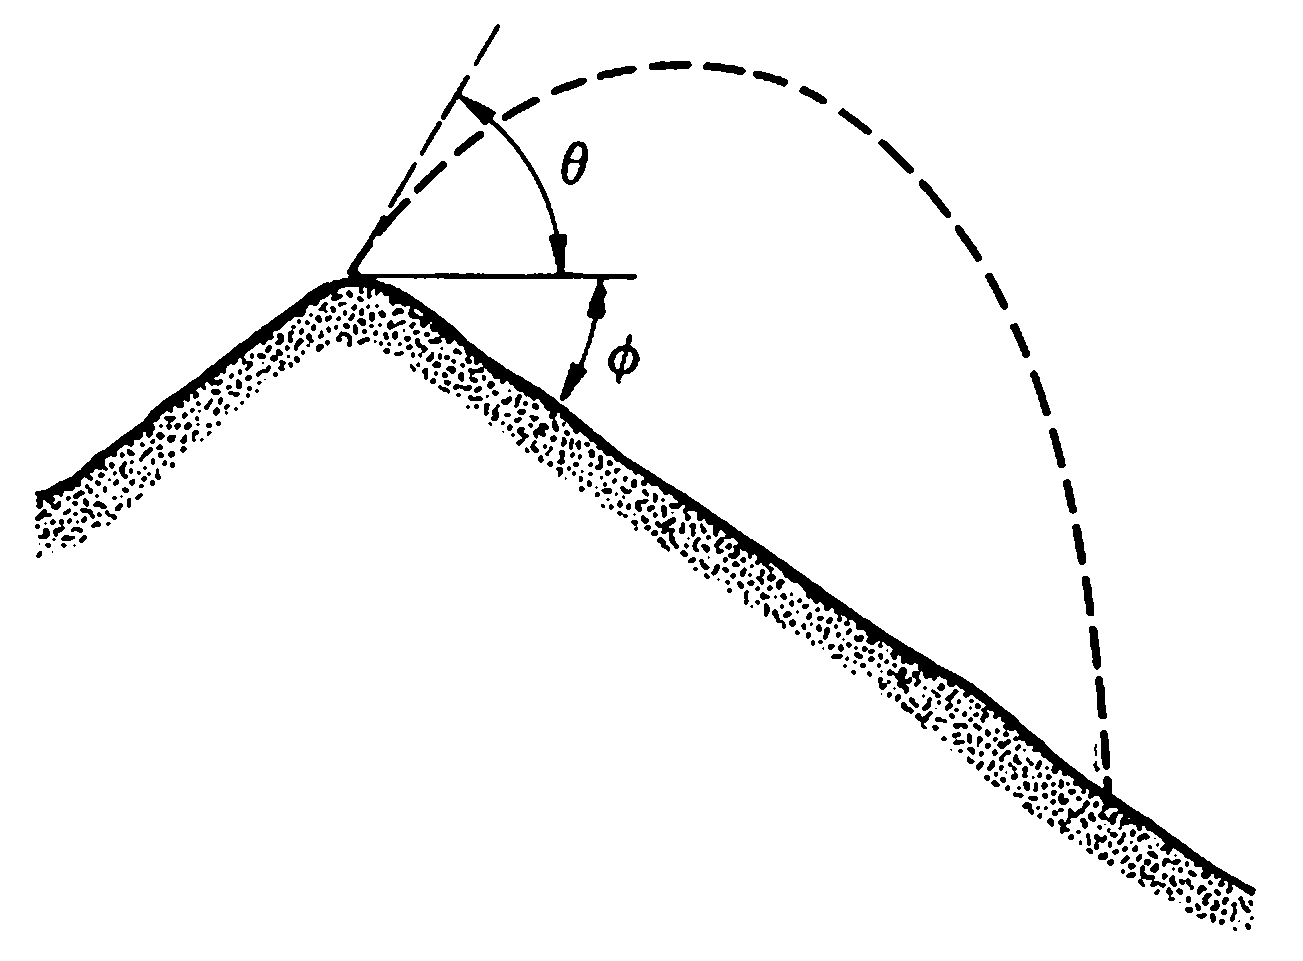
\includegraphics[width=0.5\textwidth]{ps01_4}\end{center}
\subsection*{Solution}
  The height of the hill, $h_h(x)$, is $-x\tan \phi$.  The acceleration of the rock, $\frac{\partial^2 \vec r(t)}{\partial t^2}$, is $-g\hat j$.  The velocity of the rock, $\frac{\partial \vec r(t)}{\partial t}$, is $(v_0\sin\theta -gt)\hat j + v_0\cos\theta \hat i$.  The position of the rock, $\vec r(t)$, is $\left(v_0 t\sin\theta -\frac{1}{2}gt^2\right)\hat j + v_0 t\cos\theta \hat i$.  The rock stops when $v_0 t\sin\theta -\frac{1}{2}gt^2 = -v_0 t \cos\theta\tan \phi$, or $v_0\sin\theta -\frac{1}{2}gt = -v_0 \cos\theta\tan \phi$.  Solving for $t$, $t = \frac{2v_0\sin\theta + 2v_0 \cos\theta\tan \phi}{g}$.  The maximal range occurs when $v_0 t\cos\theta = v_0 \frac{2v_0\sin\theta\cos\theta}{g} + v_0\frac{2v_0 \cos^2\theta\tan \phi}{g} = \frac{v_0^2\sin2\theta + 2v_0^2 \cos^2\theta\tan \phi}{g}$ is maximal, which occurs when $\frac{2v_0^2\cos2\theta + 4v_0^2 \cos\theta\sin\theta\tan \phi}{g} = 0$, or $\cos2\theta\cos\phi + \sin2\theta\sin \phi = \cos(\phi - 2\theta) = 0$.  This is true when $\phi - 2\theta = 2k\pi \pm \frac{\pi}{4}$ for $k\in\mathbb{Z}$.  Then, the optimal angle is $\frac{\phi}{2} - \frac{\pi}{8}$.
\end{document}
